\section{Results}
\label{sec:results}

\subsection{Accuracy Across Budget Conditions}
\label{sec:results:accuracy}

\Tabref{tab:main_results} presents accuracy across all dataset--budget combinations. The length--accuracy relationship varies dramatically by task.

\begin{table}[t]
\centering
\caption{Accuracy (\%) by dataset and budget condition with 95\% bootstrap confidence intervals. Best fixed-budget result per dataset in \textbf{bold}. The adaptive strategy uses confidence-based escalation from \shortbudget to \longbudget.}
\label{tab:main_results}
\resizebox{\textwidth}{!}{%
\begin{tabular}{@{}lcccccc@{}}
\toprule
\textbf{Dataset} & \nocot & \shortbudget & \medbudget & \longbudget & \unconst & \adaptive \\
\midrule
\math & 46.2 {\scriptsize [35--58]} & 62.5 {\scriptsize [51--73]} & 70.0 {\scriptsize [59--79]} & 71.2 {\scriptsize [61--81]} & \textbf{77.5} {\scriptsize [69--86]} & 71.2 \\
\gsmk & 92.5 {\scriptsize [86--98]} & \textbf{93.8} {\scriptsize [88--99]} & 90.0 {\scriptsize [84--96]} & 91.2 {\scriptsize [85--96]} & \textbf{93.8} {\scriptsize [88--99]} & 91.2 \\
\mmlupro & 62.5 {\scriptsize [51--73]} & 72.5 {\scriptsize [63--83]} & 75.0 {\scriptsize [65--84]} & 77.5 {\scriptsize [68--86]} & \textbf{78.8} {\scriptsize [69--88]} & 71.2 \\
\musr & 10.3 {\scriptsize [4--18]} & 5.1 {\scriptsize [1--10]} & 14.1 {\scriptsize [6--22]} & \textbf{21.8} {\scriptsize [13--31]} & 20.5 {\scriptsize [13--30]} & 7.7 \\
\bottomrule
\end{tabular}
}
\end{table}

\para{MATH and MMLU-Pro: monotonically increasing.} On both \math and \mmlupro, accuracy increases with each budget level. For \math, accuracy rises from 46.2\% (\nocot) to 77.5\% (\unconst), a 31.3 percentage point gain. The jump from \nocot to \medbudget is statistically significant ($p{=}0.002$), while the gain from \medbudget to \unconst is not ($p{=}0.28$), indicating diminishing returns. \mmlupro follows a similar pattern (62.5\%$\rightarrow$78.8\%).

\para{GSM8K: flat.} On \gsmk, accuracy is near-ceiling across all conditions ($90{-}93.8\%$), with no statistically significant differences between any pair of budgets. This confirms that easy tasks within the model's capability show no benefit from extended reasoning.

\para{MuSR: non-monotonic.} On \musr, we observe the hypothesized non-monotonic pattern. \shortbudget (5.1\%) is \emph{worse} than \nocot (10.3\%), suggesting that forcing brief reasoning can be actively harmful. Accuracy then climbs to peak at \longbudget (21.8\%) before declining slightly at \unconst (20.5\%). This is the only dataset exhibiting the inverted-U shape.

\Figref{fig:accuracy_curves} visualizes these accuracy curves across all budget conditions, and \figref{fig:accuracy_tokens} shows accuracy as a function of actual token usage.

\begin{figure}[t]
    \centering
    \begin{subfigure}[b]{0.48\textwidth}
        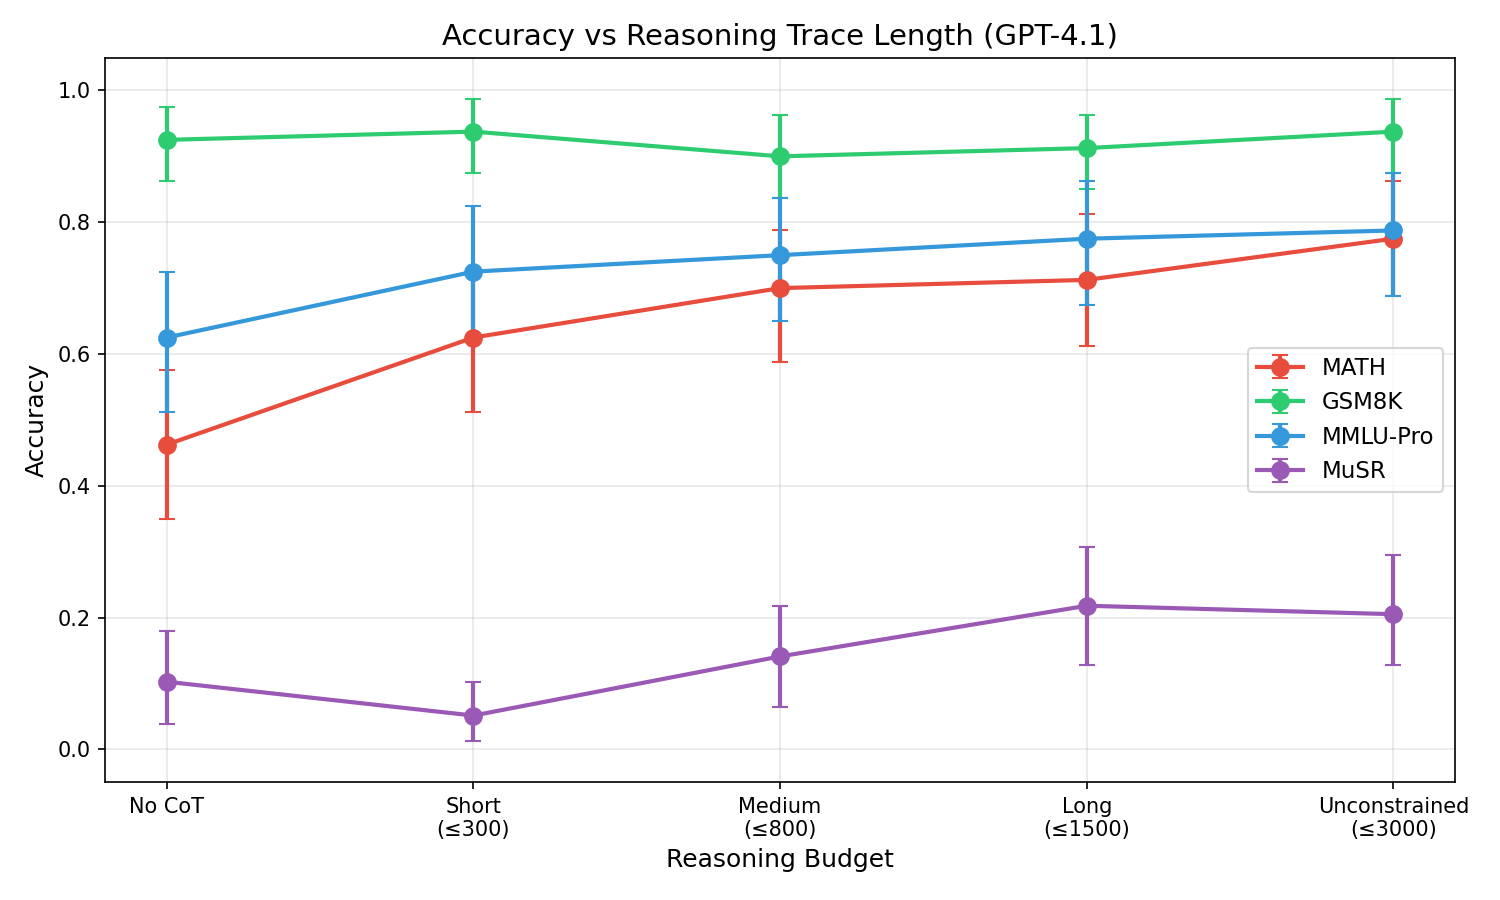
\includegraphics[width=\textwidth]{figures/accuracy_curves.png}
        \caption{Accuracy vs.\ budget condition}
        \label{fig:accuracy_curves}
    \end{subfigure}
    \hfill
    \begin{subfigure}[b]{0.48\textwidth}
        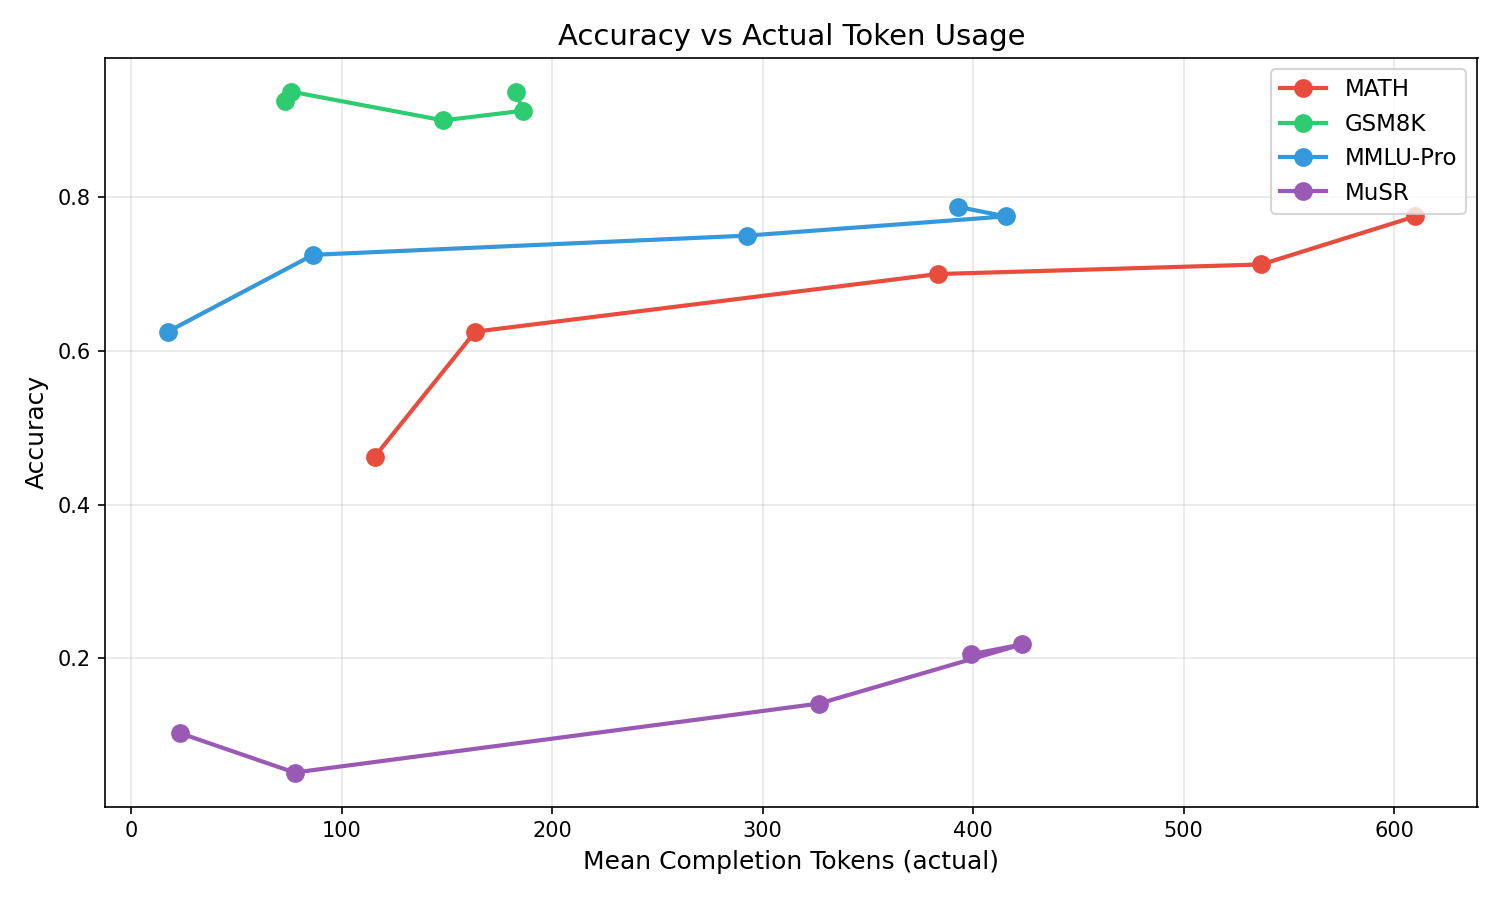
\includegraphics[width=\textwidth]{figures/accuracy_vs_tokens.png}
        \caption{Accuracy vs.\ actual token count}
        \label{fig:accuracy_tokens}
    \end{subfigure}
    \caption{Length--accuracy curves by dataset. \figleft Accuracy across five budget conditions. \math and \mmlupro increase monotonically; \gsmk is flat; \musr shows a non-monotonic pattern with \shortbudget performing worse than \nocot. \figright Accuracy plotted against mean actual completion tokens, showing that the \longbudget and \unconst conditions produce similar token counts despite different allocated budgets.}
    \label{fig:curves}
\end{figure}

\subsection{Token Usage and Self-Regulation}
\label{sec:results:tokens}

\Tabref{tab:tokens} reports mean actual token counts. A notable finding is that the model \emph{self-regulates} its output length: the \longbudget (max 1500) and \unconst (max 3000) conditions produce similar actual token counts (${\sim}400{-}600$ tokens), suggesting the model reaches a natural stopping point regardless of the allocated budget ceiling.

\begin{table}[t]
\centering
\caption{Mean actual completion tokens by dataset and budget condition. Despite large differences in allocated budgets (150--3000), actual usage converges for the \longbudget and \unconst conditions.}
\label{tab:tokens}
\begin{tabular}{@{}lccccc@{}}
\toprule
\textbf{Dataset} & \nocot & \shortbudget & \medbudget & \longbudget & \unconst \\
\midrule
\math & 116 & 163 & 383 & 537 & 610 \\
\gsmk & 73 & 76 & 148 & 186 & 183 \\
\mmlupro & 17 & 86 & 293 & 415 & 393 \\
\musr & 23 & 78 & 327 & 423 & 399 \\
\bottomrule
\end{tabular}
\end{table}

On \gsmk, the model uses very few tokens even when given unconstrained budgets (${\sim}183$ tokens at \unconst), reflecting its ease with the task. In contrast, \math elicits longer traces (${\sim}610$ tokens at \unconst), consistent with the higher difficulty.

\subsection{Robustness Gap Analysis}
\label{sec:results:gap}

\Figref{fig:robustness} shows the \robgap ($\Delta_{\text{rob}} = \text{Acc}_{\text{MATH}} - \text{Acc}_{\text{OOD}}$) across budget conditions. The behavior differs by OOD benchmark:

\begin{figure}[t]
    \centering
    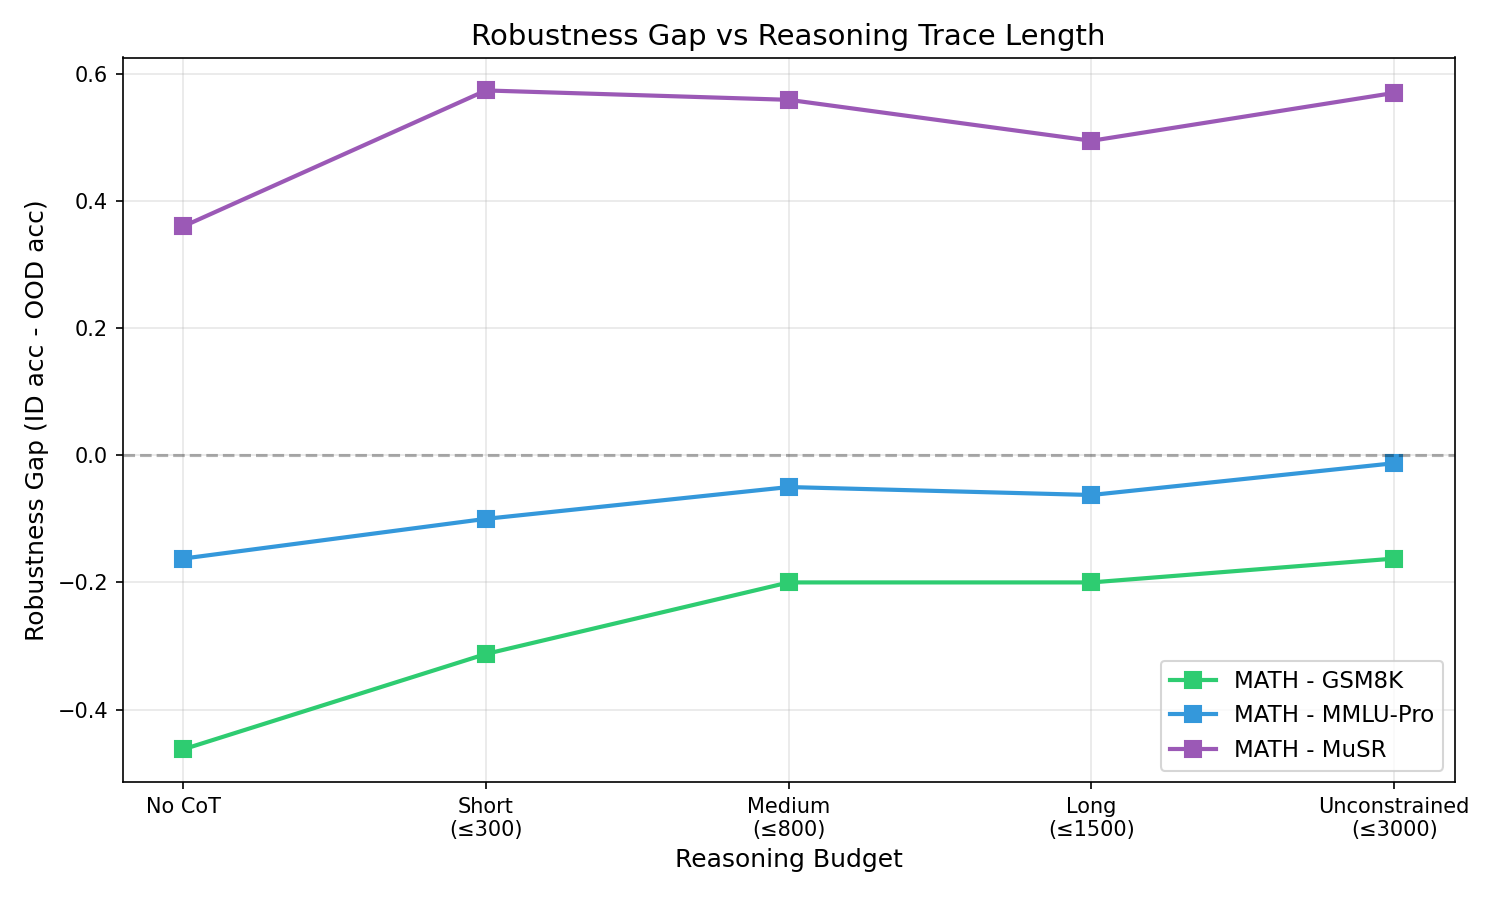
\includegraphics[width=0.7\linewidth]{figures/robustness_gap.png}
    \caption{Robustness gap ($\text{Acc}_{\text{MATH}} - \text{Acc}_{\text{OOD}}$) by budget condition. The MATH--GSM8K gap is negative because GSM8K accuracy exceeds MATH. The MATH--MuSR gap is non-monotonic, widening at \shortbudget before narrowing at \longbudget.}
    \label{fig:robustness}
\end{figure}

\para{MATH--GSM8K gap.} This gap is negative (GSM8K outperforms MATH) and narrows with longer traces, from $-0.46$ at \nocot to $-0.16$ at \unconst, reflecting MATH accuracy catching up as reasoning effort increases.

\para{MATH--MMLU-Pro gap.} Follows a similar narrowing pattern ($-0.16$ at \nocot to $-0.01$ at \unconst), with longer traces closing the gap almost entirely.

\para{MATH--MuSR gap.} Exhibits a non-monotonic pattern. The gap \emph{widens} from 0.36 (\nocot) to 0.57 (\shortbudget) as short reasoning hurts MuSR more than MATH. It then narrows to 0.50 (\longbudget) before widening again to 0.57 (\unconst). The gap is minimized at the \longbudget condition, partially supporting our hypothesis that moderate-length reasoning optimizes robustness.

\subsection{Confidence Calibration}
\label{sec:results:calibration}

\Figref{fig:calibration} presents confidence calibration results. We find a stark divergence between ID and OOD calibration quality.

\begin{figure}[t]
    \centering
    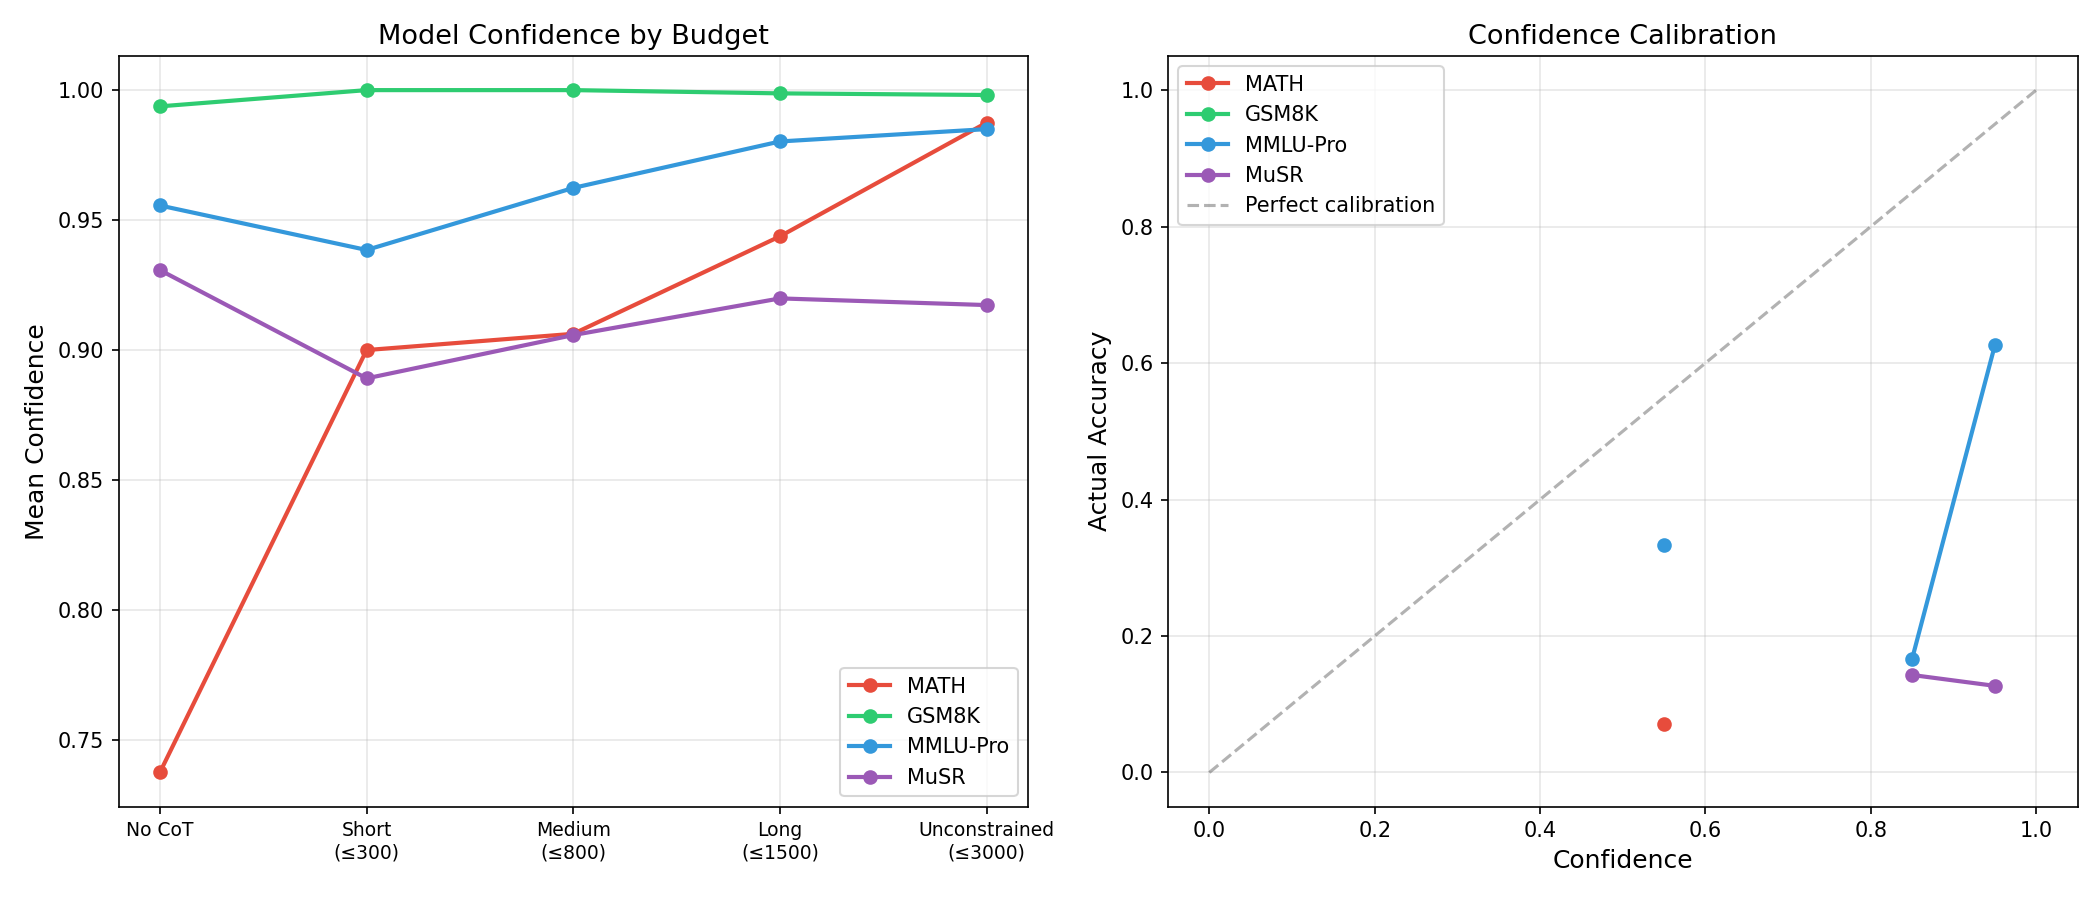
\includegraphics[width=0.7\linewidth]{figures/confidence_calibration.png}
    \caption{Confidence calibration by dataset. Spearman $\rho$ between model-expressed confidence and correctness. Confidence is a strong signal on \math ($\rho{=}0.633$, $p{<}0.0001$) but completely uninformative on \musr ($\rho{=}-0.017$, $p{=}0.74$).}
    \label{fig:calibration}
\end{figure}

\begin{table}[t]
\centering
\caption{Confidence--correctness Spearman correlations by dataset. Model confidence is well-calibrated in-distribution but catastrophically miscalibrated on the hardest OOD benchmark.}
\label{tab:calibration}
\begin{tabular}{@{}lcc@{}}
\toprule
\textbf{Dataset} & \textbf{Spearman $\rho$} & \textbf{$p$-value} \\
\midrule
\math & 0.633 & $< 0.0001$ \\
\gsmk & 0.304 & $< 0.0001$ \\
\mmlupro & 0.301 & $< 0.0001$ \\
\musr & $-0.017$ & 0.74 \\
\bottomrule
\end{tabular}
\end{table}

On \math, confidence is a strong predictor of correctness ($\rho{=}0.633$), making it a viable signal for adaptive reasoning depth. On \gsmk and \mmlupro, the correlation is moderate ($\rho{\approx}0.30$). On \musr, however, the correlation is essentially zero ($\rho{=}-0.017$, $p{=}0.74$): the model reports high confidence ($>75\%$) on nearly all questions despite achieving only 5--22\% accuracy. This systematic overconfidence on hard OOD tasks represents a fundamental failure mode for any confidence-based adaptive strategy.

\subsection{Adaptive Strategy Evaluation}
\label{sec:results:adaptive}

The adaptive two-pass strategy (escalate from \shortbudget to \longbudget if confidence $< 75\%$) shows a clear split:

\para{Success on MATH.} On \math, the adaptive strategy achieves 71.2\% accuracy (matching \longbudget) while using only 366 mean tokens versus 537 for \longbudget---a 32\% token reduction. This demonstrates that confidence-based escalation is viable in-distribution.

\para{Failure on MuSR.} On \musr, the adaptive strategy achieves only 7.7\%---worse than all fixed budgets at \medbudget or above. The failure mode is clear: only 1 of 78 questions triggers escalation because the model is overconfident despite being wrong. The strategy defaults to \shortbudget answers, which we have shown are the worst-performing condition on this benchmark.

\subsection{Token Efficiency}
\label{sec:results:efficiency}

\Figref{fig:efficiency} shows accuracy per token across conditions.

\begin{figure}[t]
    \centering
    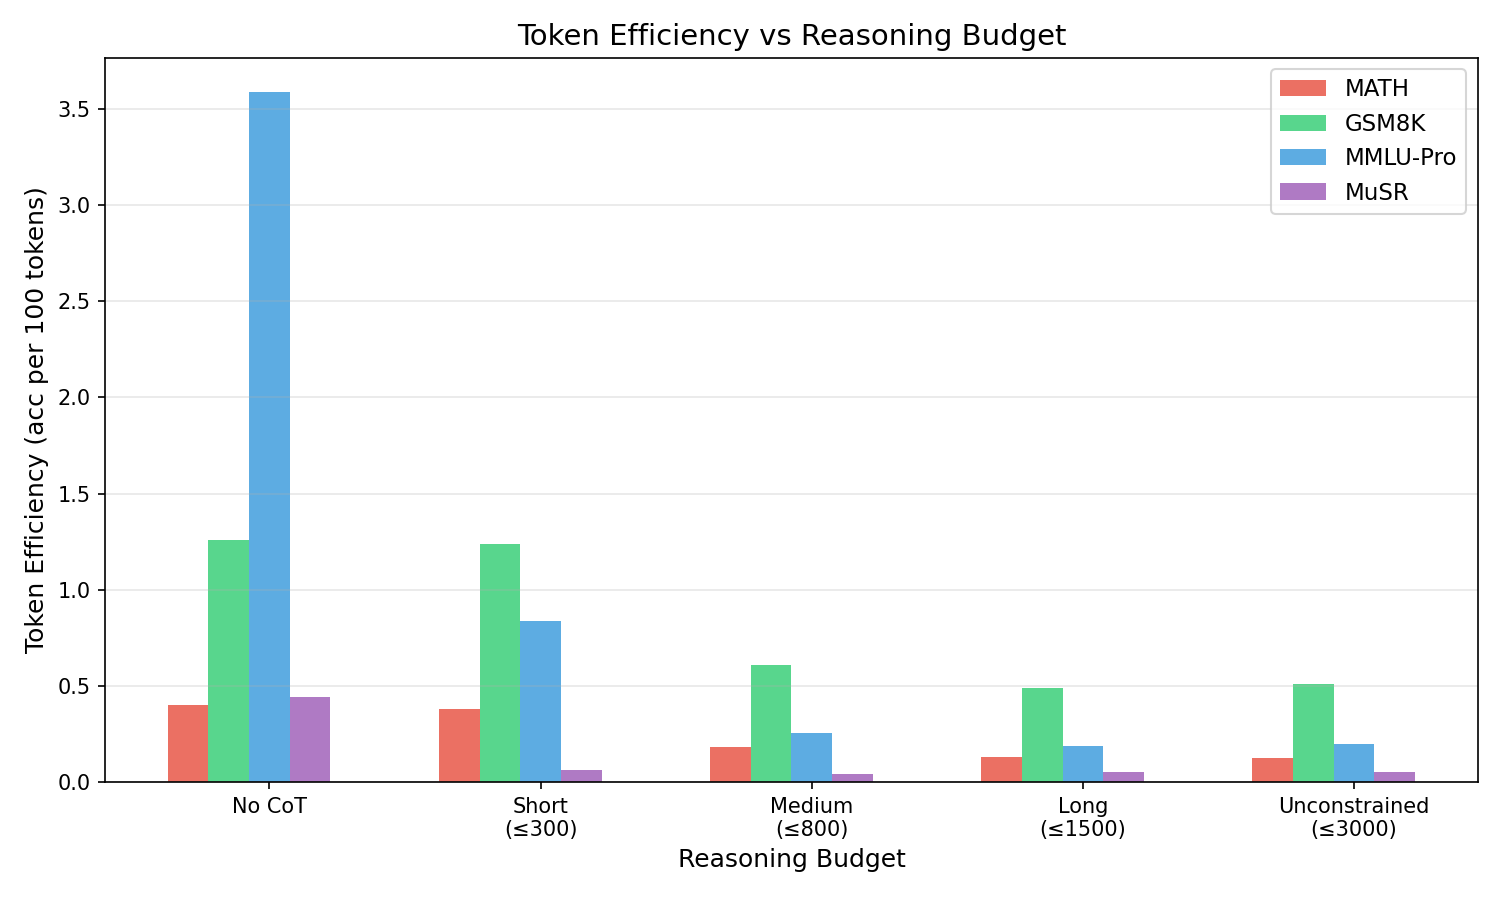
\includegraphics[width=0.7\linewidth]{figures/token_efficiency.png}
    \caption{Token efficiency (accuracy / mean tokens $\times$ 100) by dataset and budget condition. On easy tasks (\gsmk), \nocot is by far the most efficient. On harder tasks, efficiency peaks at moderate budgets before declining.}
    \label{fig:efficiency}
\end{figure}

On \gsmk, \nocot achieves the highest token efficiency because near-ceiling accuracy is reached with minimal tokens. On \math, the \shortbudget condition is most efficient (balancing accuracy gain against token cost), though absolute accuracy continues to improve with longer traces. On \musr, the \longbudget condition is most efficient, achieving the best balance of accuracy and token cost. These results suggest that optimal token allocation depends on both the task and the desired accuracy--efficiency trade-off.

\subsection{Difficulty Interaction}
\label{sec:results:difficulty}

\Figref{fig:difficulty} shows the interaction between \math difficulty level and budget condition.

\begin{figure}[t]
    \centering
    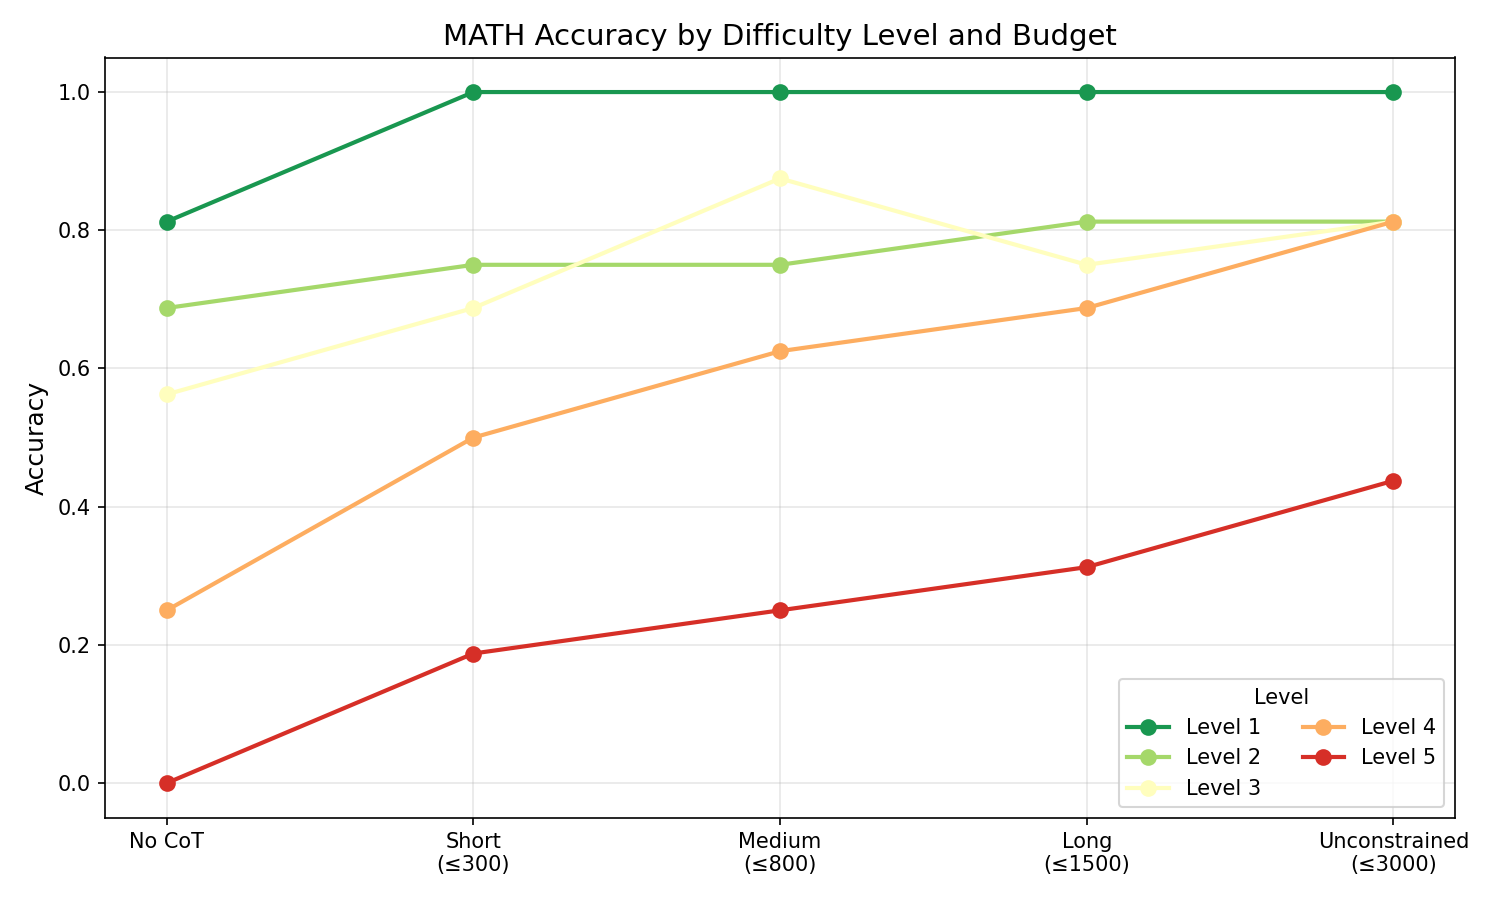
\includegraphics[width=0.7\linewidth]{figures/difficulty_interaction.png}
    \caption{Accuracy on \math by difficulty level and budget condition. Harder problems (Level 5) show the largest absolute benefit from longer reasoning, while easier problems (Level 1--2) see minimal improvement beyond \shortbudget.}
    \label{fig:difficulty}
\end{figure}

The benefit of longer reasoning is concentrated on harder problems. For Level 1--2 problems, \shortbudget achieves near-ceiling accuracy, while Level 5 problems show continued improvement through the \unconst condition. This difficulty-dependent effect is consistent with the task-level patterns we observe: easy tasks saturate quickly, while hard tasks benefit from extended reasoning up to a point.
